\documentclass[12pt]{article}
\usepackage[T1]{fontenc}
\usepackage[utf8]{inputenc}
\usepackage[usenames,dvipsnames]{xcolor}
\usepackage{minted}
\usepackage{setspace}
\usepackage{caption, newfloat}
\usepackage{upquote}
\usepackage{graphicx}

\renewcommand{\contentsname}{Topics}
\renewcommand*{\addcontentsline}[3]{\addtocontents{#1}{\protect\contentsline{#2}{#3}{}}}

\setlength{\marginparwidth}{1.2in}
\let\oldmarginpar\marginpar
\renewcommand\marginpar[1]{\-\oldmarginpar[\raggedleft\footnotesize #1]%
{\raggedright\footnotesize #1}}

\newcommand{\todo}[1]{\marginpar{\color{red} #1}}

\newcommand{\adj}[1]{{\color{blue} #1}}

\newcommand{\say}[1]{{\color{magenta} #1}}

\renewcommand{\tt}[1]{\texttt{#1}}

\newenvironment{code}[3][false]
 {
  \VerbatimEnvironment

  \begin{lstlisting}
  \caption{#3}
  \begin{minted}[linenos=#1]{#2}}
 {
  \end{minted}
  \end{lstlisting}
 }


\DeclareFloatingEnvironment[placement={H}]{lstlisting}[Example][List of Listings]
\captionsetup[lstlisting]{box=colorbox,boxcolor=RoyalBlue,font={color=white, bf},labelsep=endash,skip=5pt}

\setlength{\headheight}{15pt}

\begin{document}

\title{Lecture 4: HTTP \& AJAX}
\author{Nick Hynes}
\date{January 21, 2014}

\maketitle

\begin{spacing}{0}
\setcounter{tocdepth}{1}
\tableofcontents
\end{spacing}

\section{Introduction to Networking}
Despite what the name may imply, this will not be a lesson on making business connections. Rather, we will be discussing how data is transferred across the network to produce what we all know and love as the World Wide Web!
\par
WWW and many other Internet applications like email and centralized file hosting/sharing (as opposed to distributed, P2P architectures like BitTorrent) operate using the \emph{client-server} model. In this model, the client---or the user's browser, in our case---sends a request for a certain file, or resource, to a server which processes the request and sends back to the client either the requested resource or a status code that explains why the request failed.
\begin{center}
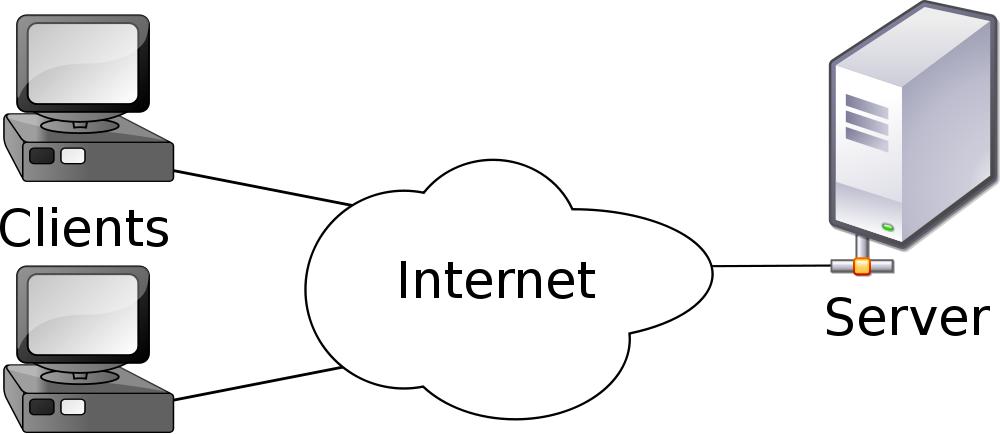
\includegraphics[scale=.25]{images/client-server.png}
\end{center}
\par
Of course, the server may perform computations based on the request parameters (e.g.\ request variables, request payload, cookies) and return a dynamically-generated page. If you use a web-service like Facebook or Gmail, then you're already familiar with this kind of server-side dynamism.


\section{HTTP(S)}
HTTP and HTTPS are the main ways HyperText is transferred over the network. HTTP stands for HyperText Transfer Protocol and, as you may already be thinking, is used to transfer documents containing HyperText. The `S' in HTTPS means Secure; HTTPS is basically encrypted HTTP.
\par
HTTP is a protocol used to request and send resources over the network. This is done by attaching an HTTP header to every request and response. Fortunately, in HTTP/1.1, the current version, these headers are in a great form for demonstration: human-readable text! The following examples are similar to the request and response headers generated every time you visit the course website.

\begin{code}[true]{http}{Requesting introjsiap.com}
GET / HTTP/1.1
Host: introjsiap.com
Connection: keep-alive
User-Agent: Mozilla/5.0 Gecko/20100101 Firefox/26.0
Accept: text/html,application/xhtml+xml,application/xml;q=0.5
Accept-Language: en-US,en;q=0.5
Accept-Encoding: gzip, deflate
If-None-Match: "80b3c-dd3-4f03251d489e7"
If-Modified-Since: "Fri, 17 Jan 2014 22:46:58 GMT"
Cache-Control: "max-age=0"
\end{code}
This header can be broken down into three main parts. On lines 1-3, the client (or, more precisely, the user-agent), specifies what resource it wants, specifically the document root of introjsiap.com (/), and how the connection should be handled after the initial transaction ends. On lines 5-7, the user-agent specifies the preferred type, language, and compression options of the requested resource; the server can use this information to \emph{negotiate} which resource to send. Finally, the fields on lines 8-10 deal with caching; since the client already has a page identified by ``80b3c-dd3-4f03251d489e7'', that was modified some time before 17/1/14, it doesn't need the server to resend it if it hasn't changed.
\par
The first portion is the most important for client-side networking, so we'll focus on that today. Line 1, itself, consists of three parts: the HTTP \emph{verb}, which defines how the server should process the request, the requested resource, specified by by a URL, and the HTTP version, which will in most cases be 1.1 (until 2.0 is adopted). The other interesting field is \texttt{Connection}. A value of \texttt{keep-alive}, as opposed to \texttt{close}, signals to the server that the TCP (socket) connection should be reused for future requests; this feature of HTTP/1.1 significantly cuts down on networking overhead.

\begin{code}[true]{http}{Here you go: introjsiap.com}
HTTP/1.1 200 OK
Connection: keep-alive
Date: Tue, 21 Jan 2014 11:11:11 GMT
Etag: "80b3c-dd3-4f03251d489e7"
Keep-Alive: timeout=5
Server: Apache/2.2.16 (Debian)
Vary: Accept-Encoding
Content-Length: 3450

<!-- page contents here (has a length of 3450 bytes) -->
\end{code}
The response headers are marginally less interesting than the request headers, so we'll be a bit more choosy with them. The most important part, by far, is on the first line; specifically the numerical status code, in this case \texttt{200}. This allows the client to determine if the request succeeded or the reason it didn't. The \texttt{Etag} field is a document version identifier used to facilitate caching. The \texttt{Content-Length} specifies how many bytes the client should read before considering the message to be finished.
\par
There are many other request and response header fields, but they should reveal themselves to you when the time comes (sounds almost mythical doesn't it?). The above examples should encapsulate all of the most important features of basic HTTP. In fact, now that you know how to formulate HTTP requests, you don't even have to use a web browser any more!

\subsection{Methods}
The following HTTP request methods, commonly referred to as verbs, are used to signal the intent of the client's request and should be implemented on the server in a reasonable (aka sane) manner.
\begin{itemize}
\item GET - Requests the specified resource. Should only retrieve data and nothing else. To send parameters to the server using this request method, use \texttt{http://theurl/?param1=value1\&param2=value2\&etc}
\item POST - Requests that the server create a new sub-resource based on the request payload. The payload is urlencoded (like the GET parameters without the ?) or JSON and is included as the body of the POST request. Don't forget to set the media type and the content length!
\item PUT - Requests that the server set or update the resource at the specified path to the contained data. This is similar to POST except that it creates/update the resource rather than a sub-resource.
\item DELETE - Deletes the specified resources.
\item HEAD - Requests only the headers (this one isn't too common)
\end{itemize}
As with most things covered thus far, this list is not complete, but is likely to be the most useful. You may satisfy your curiosity, however, by following the link in \emph{Additional resources}.

\subsection{Status codes}
\begin{center}
  \begin{tabular}{| c | c | p{7.06cm} |}
    \hline
    \textbf{Status code} & \textbf{What it means} & \textbf{When it's used} \\
    \hline
    200 & OK & Everything went well and the server returned the requested page. Everyone is happy. \\
    \hline
    301 & Moved permanently & The resource previously located at the requested URL has moved to another URL. Use this in conjunction with the \texttt{Location} header field to get the user-agent to redirect.\\
    \hline
    400 & Bad request & The client sent an ill-formatted request and the server doesn't know what else to do. \\
    \hline
    401 & Unauthorized & The user needs to authenticate to gain access to the resource. This is used with HTTP authentication (not form-based auth). \\
    \hline
    403 & Forbidden & The user does not have permission to make the request. \\
    \hline
    404 & Not found & The server couldn't find the requested resource \\
    \hline
    500 & Internal server error & The server had an error and could not complete the request \\
    \hline
  \end{tabular}
\end{center}
There is a link to a complete list of HTTP status codes in the \emph{Additional resources} section. While those listed should provide all of the basic, required functionality, there might be a status code that is more descriptive and appropriate for your application.

\subsection{REST}
The combination of HTTP methods, cookies, status codes, headers, and authentication provides a particularly rich medium for creating scalable, modular, high-performance web-applications. These may be buzzwords, but the underlying concept is sound.
\par
REST is an acronym for Representational State Transfer. Essentially, REST defines a client-server application model in which the client sends everything the server needs to fulfill the request with each request. This is equivalent to saying that the server does not store any sort of session data for the user. It is immediately obvious that this, along with improved caching ability, reduces the server's memory and disk space usage (at the cost of increased bandwidth and possibly latency [which can be mitigated by caching]). Additionally, resources under the REST model are located at sane URLs and are operated on using the HTTP verbs. For example, if I wanted to create a new user for my social networking application, I could send a POST request with the user's data to https://cebook.com/users (drop the `thefa', it's cleaner). The server could then return a descriptive status code that can be interpreted on the client-side to notify the user the result.

\subsection{HTTP vs HTTPS}
Whereas HTTP transactions are conducted using plaintext, those of HTTPS are encrypted using TLS (Transport Layer Security) or the less-secure SSL (Secure Sockets Layer). This prevents eavesdroppers from determining the contents of HTTP traffic. This is particularly useful for online shopping and banking and preventing the government from spying on you, among other things. While HTTPS has a small amount of performance overhead, the benefits provided by HTTPS, which also include verification of the server's identity, are sufficient reason to always use it. In fact, encrypting data using TLS is a requirement of HTTP/2.0
\par
If you think of the network as a stack (like pancakes), you have, from top to bottom, the application layer, the transport layer, the internet layer, and the link layer. HTTP and HTTPS operate on the application layer, so there's really no need to deal with the rest of the IP suite at this point (although it's really, really interesting!).
\par
The application layer is concerned with the transmission of abstract, application-specific data, as opposed to getting the data from point A to point B. HTTP operates near the top of this layer and, of course, provides a way to request and send hypertext and related resources. Here's the gist of what happens during a generic HTTP exchange: 
\begin{enumerate}
\item The client prepares an HTTP request for a certain resource
\item The HTTP request, now treated as arbitrary data, travels down the client's networking stack and is sent over the network to the server
\item The request travels up the network stack of the server and is processed by a program that understands HTTP
\item The server generates an HTTP response
\item The response travels down the network stack of the server and up the stack of the client
\item The HTTP transaction is now complete
\end{enumerate}
TLS sits at the bottom of the application layer so that when HTTP traffic passes through it from either direction, it is either encrypted or decrypted using a session secret (this is also a really good read. The Wikipedia diagram for Diffe-Hellman key exchange is one of my favorite diagrams). Practically, this means that once TLS is established, HTTP can proceed as usual.


\section{AJAX}
Woohoo! Now for the fun part: using JavaScript to make HTTP requests. However, before we dive into AJAX (not the detergent), let me relate to you a tale of the pre-AJAX web, circa 2006.
\begin{quote}
``In a world where making a small change to a web page required a complete reload of the page, along with yet another request to the server, the user experience was comparatively bad by today's standards.
\par
Imagine submitting a form\ldots\ and being sent a new web page. The screen might even flash as the page reloads! *gasp* Oh, the horror!''
\end{quote}
AJAX remedies all of these problems as it allows an already-loaded page to make further requests of the server without actually reloading the page. Additionally, like JS event handlers, the responses to these AJAX requests are (read: should be) processed \emph{asynchronously} using callback functions; this allows the web-application to maintain a responsive user-interface and submit further AJAX requests. Thus, AJAX forms the basis of the modern, responsive web-application.
\par
The acronym AJAX technically stands for Asynchronous Javascript And XML, but basically everything \emph{but} XML is sent using it. If you're sending XML, then that's fine, too, but my only question is ``\emph{why?}'' There are infinitely less verbose serialization formats available.

\subsection{JSON}
Before covering the AJAX methods, it will be useful to re-introduce our old friend, the JavaScript Object, as a powerful and convenient method of serializing data, that is, converting it into a form that can be transferred over the wire and reconverted on the other end. The benefit of using JSON is that it's much, much less verbose than XML (saves bandwidth) and can be used by JavaScript much more easily since JSON can be parsed directly into a JavaScript object that can be manipulated using the usual methods. Here's an example of JSON in case you've forgotten:
\begin{code}{json}{An example on JSON}
[
  {
    "user": "A user",
    "message": "Hey, how's it going?"
    "timestamp": 123456789
  },
  {
    "user": "Another user",
    "message": "nm, bro, just chillin",
    "timestamp": 987654321
  }
]
\end{code}
Note that the keys are double-quoted Strings and the values are JavaScript Objects (including double-quoted Strings, Arrays, Numbers, Booleans, and generic Objects).
\par
When transferring JSON from the server, it is generally a good idea to specify the \texttt{Content-Type} of the response as \texttt{application/json} so that the client can handle it appropriately and the server can compress the file to the best of its abilities.
\begin{Verbatim}[frame=single]
//To convert a [non-circular] Object to JSON
JSON.stringify(theObj);

//To convert JSON to an Object
JSON.parse(theObj);
\end{Verbatim}

\subsection{``Native''}
\begin{code}[true]{javascript}{AJAX Using the XHR Object}
var req = new XMLHttpRequest();

var contentLoaded = function() {
  //this is the response object
  if(this.status === 200) {
    console.log(this.responseText); //"Hello, world!"
  } else {
  console.log("Error: "+this.status);
  }
}

req.addEventListener("onload", contentLoaded);
//could also use req.onload = contentLoaded

req.open("GET", "helloworld.txt", true);
req.send();
console.log("Request sent"); //"Request sent"
\end{code}
This example is slightly more concise than it would have been if support for early versions of IE were needed, but if you're lucky, this should never be the case.
\par
On the first line, we create a new XMLHttpRequest (or XHR) object. We then assign it a listener for its \emph{load} event, which is triggered when the response is received. Next, the XHR object is ``opened,'' which essentially means that its request details are set. Finally, the XHR is sent to the server and patiently awaits a response.
\par
While this is about as complicated as AJAX gets, the XHR object provides a number of methods that can be used to vastly increase its utility.
\subsubsection*{XHR object functions}
\begin{itemize}
\item getResponseHeader(String header) -- returns the value of the requested header or \texttt{null} if not set
\item \texttt{open(method, URL, [Boolean async], [user], [password])} -- \\ initializes a request of type \texttt{method}, to be sent to \texttt{URL}. If the optional \texttt{async} is true, then the XHR object's callbacks will be run when the response is received. Otherwise, all scripts on the page will block until the request is handled (This is generally a BAD IDEA\texttrademark). The optional Strings, \texttt{username} and \texttt{password} are mainly used for HTTP Basic auth (only transmit this over a secure network!).
\item setRequestHeader(String headerFieldName, String headerValue) -- sets the value of the specifieed request header field
\item send([(String|Blob) data]) -- Sends the request to the server with the body of the request containing the contents of the \texttt{data} argument. The Blob (Binary Large OBject) format is used when transferring binary data, like file uploads.
\end{itemize}

\subsubsection*{XHR object properties and events}
\begin{itemize}
\item progress event -- fired when download progress changes
\item load event -- fired when the response is loaded
\item error event -- fired when the request fails
\item abort event -- fired when the request is aborted [by the user]
\\
\item response -- the response parsed according to its content-type (of either text, JSON, Document (as in HTML Document), Blob, or ArrayBuffer) or \texttt{null} if the request did not succeed
\item responseType -- the content-type of the response (text, JSON, Document, Blob, or ArrayBuffer)
\item responseText -- the response text or \texttt{null} if the request did not succeed
\item responseXML -- the response XML or \texttt{null}
\item status -- the HTTP status code
\item statusText -- the text returned with the status code (e.g. OK for 200 OK)
\end{itemize}

\subsubsection*{Some things to watch out for}
\begin{itemize}
\item callback functions must be registered before calling \texttt{send}
\item when sending data using the argument of the \texttt{send} function, be sure to set the \texttt{Content-Type} and \texttt{Content-Length} request headers
\item the \texttt{setRequestHeader} method must be called after \texttt{open} but before \texttt{send}
\end{itemize}

\subsection{jQuery}
\subsubsection*{\$.ajax}
The jQuery AJAX function is the ``low-level interface'' for the rest of the jQuery AJAX functions.
\begin{Verbatim}[frame=single]
$.ajax(URL, [settings]); //method defaults to GET

$.ajax(settings);
\end{Verbatim}

The \texttt{settings} object passed to the jQuery \texttt{ajax} function defines all of the properties and behaviors of the request. Here's a list of some of the more interesting settings. These are all optional, by the way (except maybe URL if not already set\ldots).
\begin{itemize}
\item url: the request URL
\item type: the HTTP method to use. Default: GET
\item async: (Boolean) true if asynchronous, false if synchronous. Default: true
\item beforeSend: function(jqXHR, settings) a function that can configure the jqXHR object and its settings before it is sent
\item statusCode: (Object) an object of Number: Function pairs that defines which functions to run if a set status code is returned
\item contentType: (String) the content type. Defaults to `application/x-www-form-urlencoded; charset=UTF-8', which is good.
\item data: (Object|String) the data to be sent to the server. An Object value will be stringified.
\item headers: (Object) an object of header field: value pairs
\item username: the HTTP authentication username
\item password: the HTTP authentication password (send this over HTTPS if not using HTTP Digest auth!)
\end{itemize}

All of the jQuery AJAX methods return a jqXHR object which is a superset of the native XHR object, so you can use them in the same ways. However, the jqXHR object has the added benefit of being a jQuery Promise object that has allows chaining of callbacks on events like \texttt{done}, \texttt{fail}, \texttt{then}, and \texttt{always}. The latter two are called when anything happens to the Promise object or after the Promise object is rejected or resolved (failed or done'd), respectively.

\begin{code}{javascript}{AJAX Using jQuery's \texttt{\$.ajax}}
$.ajax("helloworld.txt")
  .done(function(data) {
  console.log(data); //"Hello, world!"
  })
  .error(function(jqXHR, statusText) {
    console.log("Error: " + statusText);
  });
\end{code}

\subsubsection*{\$.get}
The \texttt{\$.get} function is simply a convenience method for \texttt{\$.ajax}.
\begin{Verbatim}[frame=single]
$.get(URL, [data], [success callback]);
//Chaining callbacks still works, but a success callback
//can be passed directly to the function
\end{Verbatim}

\subsubsection*{\$.getJSON}
This method is a convenience method for \texttt{\$.get}. A convenience method of a convenience method. How convenient! The difference is that the \texttt{data} parameter passed to the callback functions is a JS object.
\begin{Verbatim}[frame=single]
$.getJSON(URL, [data], [success callback]);
//Chaining callbacks still works, but a success callback
//can be passed directly to the function
//callback takes format of (data, textStatus, jqXHR)
\end{Verbatim}

\subsubsection*{\$.getScript}
This method GETs a JavaScript from the server and then executes it.
\begin{Verbatim}[frame=single]
$.getScript(URL, [success callback]);
//Chaining callbacks still works, but a success callback
//can be passed directly to the function
//callback takes format of (script, textStatus, jqXHR)
\end{Verbatim}

\subsubsection*{\$.post}
Like a GET request except POST (so it's not really like a GET request at all then, is it?).
\begin{Verbatim}[frame=single]
$.post(URL, [data], [success callback]);
//Chaining callbacks still works, but a success callback
//can be passed directly to the function
//callback takes format of (script, textStatus, jqXHR)
\end{Verbatim}

\subsubsection*{jQueryFormObject.serialize()}
Serializes a jQuery object that contains a form and returns a urlencoded String. This is very useful for sending form data using \texttt{\$.post}.

\end{document}